\setcounter{page}{1}
\section*{Zielsetzung}

In dem Versuch V703 sollen die Charakteristika eines
Geige-Müller-Zählrohr untersucht werden.
Unter diese Fallen zum Beispiel die
Totzeit und die Untersuchung von Nachentladungen.

\section{Theorie}

\subsection{Funktionsweise eines Geiger-Müller-Zählrohr}
Ein Geiger-Müller-Zähler besteht grundsätzlich aus einem
Kathodenzylinder (negativ geladen) und einem Anodendraht (positiv geladen) (vgl. Abbildung \ref{fig: schematischer_aufbau}).
Zwischen Anode und Kathode befindet sich ein Gasgemisch (bestehend aus einem Edelgas
und Alkohldampf).
\begin{figure}
  \centering
  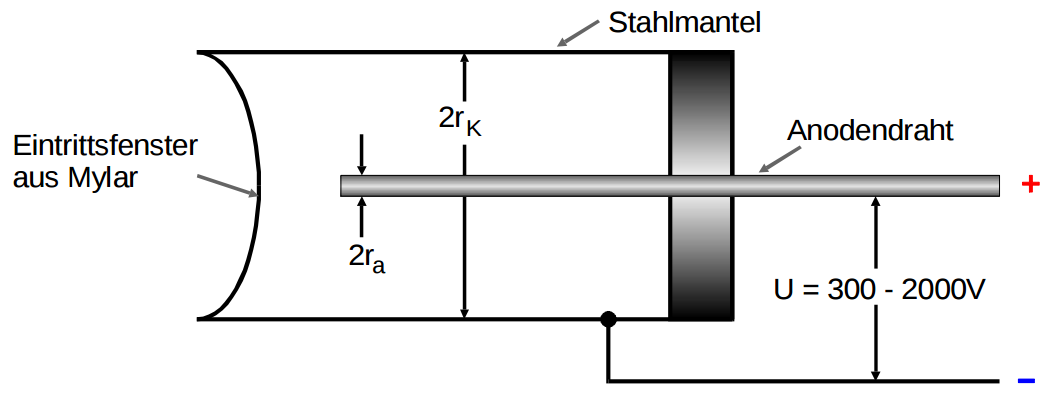
\includegraphics[width=0.6\textwidth]{bilder/geiger_.png}
  \caption{Schematische Darstellung eines Geiger-Müller-Zählrohrs \cite{anleitung703}.}
  \label{fig: schematischer_aufbau}
  \end{figure}
Durch Anlegen einer Spannung ($300-\SI{2000}{\volt}$) entsteht ein elektrisches
Feld im inneren des Zylinders. Auf der Voderseiter eines Geiger-Müller-Zählrohrs
befindet sich ein Eintrittsfenster aus Mylar. Dieses ermöglicht es selbst $\alpha$-
Strahlung in das Zählrohr einzutreten. Gelangt ionisiernde Strahlung
in das Zählrohr, so ionisiert diese das Gasgemisch. Die freigeschlagenden
Elektronen, können je nach anliegender Spannung, weitere Atome ionisieren.
Die dadurch entstehende Elektronenlawine (als Townsend-Lawine bezeichnet) gelangt zu der Anode und erzeugt so
einen Strom. Der Strom wird mittels einem Verstärker verstärkt und an ein
Zählgerät weitergeleitet. Wie Oben angesprochen hängt die Anzahl der regrestierten
Elektronen von der anliegenden Spannung ab (vgl. Abbildung \ref{fig:teilchen_spannung}).
\begin{figure}
  \centering
  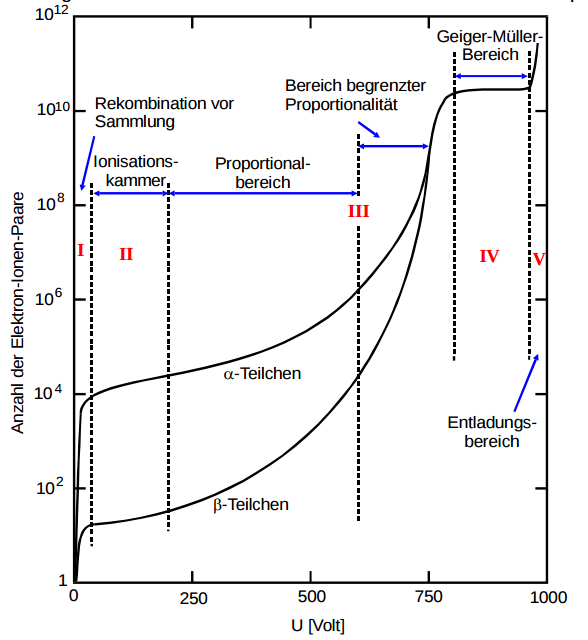
\includegraphics[width=0.6\textwidth]{bilder/diagramm.png}
  \caption{Anzahl der gemessen Teilchen pro Zeit bei unterschiedlichen Spannugen \cite{anleitung703}.}
  \label{fig:teilchen_spannung}
\end{figure}
Denn bei einer zu geringen Spannung
gehen die meisten Elektronen durch Rekombination verloren. Dreht man die Spannung weiter auf
kommt man in den \emph{Arbeitsbereich einer Ionisationskammer}, dieser funktioniert aber nur bei
bei Stahlungen mit hoher Intensitäten. Durch eine weiter Erhöhung der Spannung gelangt man
in den sogenannten \emph{Propotionalbereich}. In diesem besitzen die Elektronen
genügend Energie, um ihrerseits weitere Atome ionisieren zu können (auch Stoßionisation genannt).
Der Vorteil in diesem Bereich liegt daran, das hier neben der Teilchenanzahl auch doe Energie
einfallenden Spannung gemessen werden kann. Bei wiederholte Erhöhung der Spannung
gelangt man in den \emph{Auslösebereich}. In diesem liegt der Arbeitsbereich des
Geiger-Müller-Zählers. In diesem Bereich besitzen die ausgelösten Elektronenlawinen
eine große Anzahl an UV-Photonen. Die Photonen können sich senkrecht zum elektrischen Feld bewegen
und lösen so Townsend-Lawine im gesamten Zählrohr aus. Der Efffekt hat eine
\emph{Totzeit} zu folge, bei dieser ist es dem Zählrohr neu eindringende Teilchen
zu messen. Begründen kann die Totzeit mit der durch die Elektronenlawine entstehenden
positiv geladenen Ionen. Da die Ionen eine größere Masse als Elektronen besitzen,
bewegen sie sich wesentlich langsamer zur Kathode, als die Elektonen
zur Anode. Dadurch entsteht in der Kammer ein Gegenfeld, welches das
elektrische Feld (erzeugt von Kathode und Anode) abschwächt.
Erst nachdem die Ionen die Kathode erreicht haben, ist eine
Regrestierung wieder möglich. Nach der Totzeit schließt sich
noch eine \emph{Erholungszeit} an. In dieser Zeit erzeugen
die an der Kathode eintrefenden Ionen neue Elektronen, die eine neue
schwächere Elektronenlawine herrvorufen kann (Nachentladung gennant). Beide Zeiten sind
in Abbildung \ref{fig: tot_und_erholungszeit} grafisch dargestellt.
\begin{figure}
  \centering
  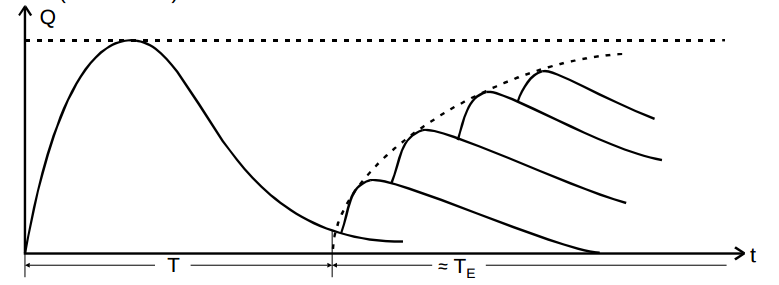
\includegraphics[width=0.6\textwidth]{bilder/totzeit.png}
  \caption{Grafische Darstellung von Tot- und Erholungszeit \cite{anleitung703}.}
  \label{fig: tot_und_erholungszeit}
  \end{figure}
Der Alkoholdampf im Gasgemisch
soll die Erholungszeit verringern. Erklärbar ist es damit, dass
die Edelgasionen die Alkoholmolekül ionisiern. Die Alkoholmoleküle
besitzen eine geringere Ionisierungsenergie und können so keine Elektronen aus
der Kathode schlagen. Zusätzlich besitzt eine Alkohlmolekül mehr Schwingungsmodie
mit verschiedenen Frequenz. Durch diese verliert das Alkohlmolekül
weitere Energie (wegen $E=\map{h}f$).

\subsection{Charakteristika des Zählrohrs}
In dem Arbeitsbereich des Geiger-Müller-Zählers erhält man einheiten
charkteristischen Verlauf der regrestierten Teilchen $N$.
Diese \emph{Charakteristik} ist in Abbildung \ref{} dargestellt.
\begin{figure}
  \centering
  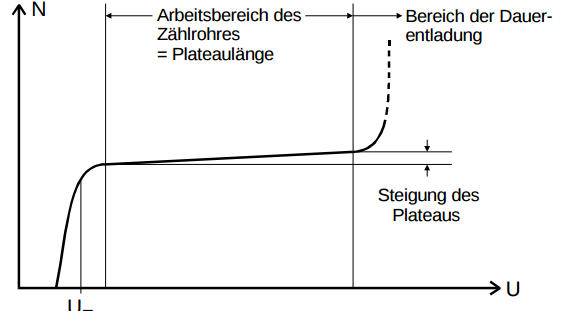
\includegraphics[width=0.6\textwidth]{bilder/plateau.png}
  \caption{Vergrößerung des Geige-Müller-Bereichs \cite{anleitung703}.}
  \label{fig: plateau}
\end{figure}
Ab der Spannung $U\ua{E}$ erreicht man den Spannungsbereich für ein
ordentliches Arbeiten des Zählrohrs. Nach dieser erhält man einen
linearen Zusammenhang zwischen $N$ und $V$, dieser wird auch als
\emph{Plateau} bezeichnet. Bei einem idealen Zählrohr besitzt der
lineare Zusammenhang eine Steigung von null. In der Realität besitzt
die Gerdade aber eine geringe Steigung. Die Steigung ist mit der oben
angesprochenden Nachentladungen erklärbar. Am Ende des Plateau nimmt die
Zahl der Nachentladungen gewaltig zu. Wird die Spannung hier noch weiter erhöht,
ist eine Zerstörung des Zählrohrs möglich.
